\documentclass[10pt, compress]{beamer}

\usetheme{m}

\usepackage{booktabs}
\usepackage[scale=2]{ccicons}
\usepackage{minted}

\usemintedstyle{trac}

\title{Ouya}
\subtitle{A Micro Games Console}
\date{\today}
\author{Fernando Ellis - Andrew Mandula - Brendan Whitfield}
\institute{Futuere}

\begin{document}

\maketitle

\section{What is it?}

    \begin{frame}{What is it?}
    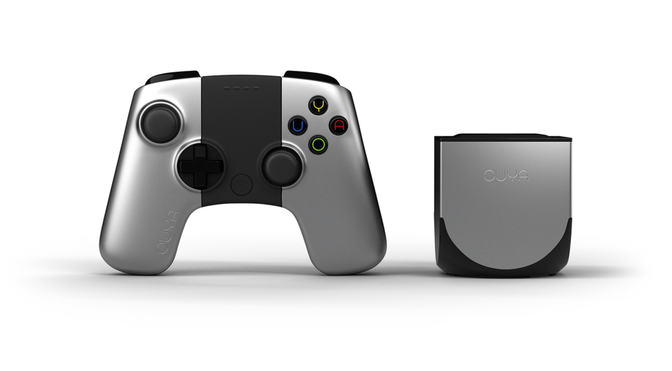
\includegraphics[width=\textwidth]{images/Ouya.png}
    \\ \begin{center}Android Powered MircoConsole \end{center}
    \end{frame}
    
    \begin{frame}{What is it?}
    \textbf{Company}
    \begin{itemize}
    \item Company: Ouya Inc.
    \item Founded: July 3, 2012
    \item HQ: Santa Monica, CA
    \item Not Publicly Traded
    \item No Acquisitions or Investments
    \item 31 Employees
    \end{itemize}
    \end{frame}
    
    \begin{frame}{What is it?}
    \textbf{Kickstarter}
    \begin{itemize}
    \item Kickstarter: August 9, 2012
    \item Funded after 8 hours
    \item Total Funding: \$8.6M
    \item Worked with XMBC, Plex, Square Enix, Bandi Namco, \& Robotoki to bring apps \& exclusive games to the platform
    \end{itemize}
    \end{frame}
    
    \begin{frame}{What is it?}
    \textbf{Investments into Ouya Inc.}
    \begin{itemize}
    \item Kickstarter: \$8.6M
    \item Series A: \$15M
    \item Alibaba: \$10M
    \end{itemize}
    \end{frame}

\section{Communications}

\begin{frame}{Communications}

\textbf{Community}
\begin{itemize}
\item IRC Channel: \#ouya irc.freenode.net (unofficial)
\item \href{https://github.com/ouya}{\alert{Github Repo}}
\item \href{https://devs.ouya.tv/developers/docs}{\alert{Documentation}}
\item \href{https://github.com/ouya/docs}{\alert{Github Documentation}}
\end{itemize}

\end{frame}

\begin{frame}{Communications}

\textbf{Social Media}
\begin{itemize}
\item \href{https://twitter.com/playouya}{\alert{Twitter: 44.3K Followers}}
\item \href{https://www.facebook.com/OUYA}{\alert{Facebook: 99,454 Likes}}
\item \href{https://instagram.com/OUYA/}{\alert{Instagram: 1,556 Followers}}
\item \href{https://www.linkedin.com/company/ouya-inc-}{\alert{Linkedin: 644 Followers}}
\item \href{https://plus.google.com/+OuyaTv/posts}{\alert{Google+: 21,141 Followers}}
\item \href{https://www.youtube.com/user/ouyas}{\alert{Youtube: 13,731 Subscribers}}
\item \href{http://www.reddit.com/r/ouya}{\alert{Reddit: 7,978 Gamers}} 
\end{itemize}

\end{frame}

\begin{frame}{Communications}

\textbf{Communication Channels}
\begin{itemize}
\item \href{https://www.ouya.tv/blog/}{\alert{Ouya official Blog}}
\item \href{https://www.ouya.tv/shout-outs/}{\alert{Ouya "Shout-outs"}}
\item \href{https://forums.ouya.tv/}{\alert{Ouya Developer Blog}}
\item \href{http://ouyaforum.com/}{\alert{Ouya unofficial Forum}}
\end{itemize}

\end{frame}

\begin{frame}{Communications}

\textbf{Conference Visits}
\begin{itemize}
\item \href{https://www.ouya.tv/gdc2014/}{\alert{GDC}}
\item \href{https://www.ouya.tv/indiecade2014/}{\alert{IndieCade}}
\end{itemize}
\textbf{Developers also visit many conferences individually, including, but not limited to:}
GDCChina, Game Connection Europe, SBGames, IndiE3, Captivate Conference, Nordic Game Conference, XOXO Conference


\end{frame}

\section{Specifications}

\begin{frame}{Specifications}
    Due to the \$100 price point, the Ouya only has specs equivalent to a mobile phone.
    \vspace{4mm}
    
    \begin{itemize}
    \item Tegra 3 - ARM Cortex-A9
    \item 1GB RAM
    \item 8GB on-board flash
    \item Wifi \& Bluetooth
    \item LAN / USB / Micro-USB / HDMI
    \end{itemize}
    
    \vspace{4mm}
    Ouya encourages hardware hacking, and making new peripherals.
\end{frame}

\begin{frame}{Specifications}
    Uses a modified version of Android
    
    \vspace{4mm}
    
    Ouya maintains several GitHub repos for a few of its open source components.

    \vspace{4mm}
    
    \begin{itemize}
    \item \href{https://github.com/ouya/ouya-sdk-examples}{\alert{ouya-sdk-examples}} - Missing License
    \item \href{https://github.com/ouya/docs}{\alert{docs}} - Missing License
    \item \href{https://github.com/ouya/ouya_1_1-kernel}{\alert{ouya\_1\_1-kernel}} - GPLv2
    \item \href{https://github.com/ouya/android_packages_apps_CMUpdater}{\alert{android\_packages\_apps\_CMUpdater}} - GPLv2
    \item \href{https://github.com/ouya/unity-2d-demo}{\alert{unity-2d-demo}} - Missing License
    \end{itemize}
\end{frame}

\begin{frame}{Summary}

  Get the source of this theme and the demo presentation from

  \begin{center}\url{github.com/matze/mtheme}\end{center}

  The theme \emph{itself} is licensed under a
  \href{http://creativecommons.org/licenses/by-sa/4.0/}{Creative Commons
  Attribution-ShareAlike 4.0 International License}.

  \begin{center}\ccbysa\end{center}

\end{frame}

\plain{}{Questions?}

\end{document}
